\section{Evaluation}
\label{sec:eval}

Our application, in addition to implementing our WiFi policies, would connect to a server and send a UDP packet every 100 milliseconds, stamped with a sequence number. To evaluate the performance our policies, we performed several experiments, with and without the appropriate policies enabled. For each experiment we inspected which packets were received to determine how many packets were dropped.

We present the setup and results from two experiments here. Each were inspired by the second and third problem situations presented. To test the Internet Access Testing policy, aproached a store with complimentary WiFi requireing authentication. For Predictive WiFi Abandonment, we left a WiFi network which was known to one of the authors to lost internet connectivity as a smartphone left [TODO: This is worded terribly][TODO: Better names for subsections...]

\subsection{Internet Access Testing - The Panera Test}
The problem of connecting to WiFi, without user intervention, that is unable to reach the internet is not cleanly measured. The impact of this issue varies on the users habits and the time spent within the network. To demonstrate this issue, as well as our solution we designed a realistic scenario to carry out. 

The experiment started across a parking lot, connected to AT\&T's HSPA network. We approached a store with public WiFi, which the phone would connect to once in range. Upon arriving at the door, we waited for 30 seconds and then attempted to access Google.com, waiting 10 seconds after successfully loading the page (including any delay from authentication).

\begin{figure}
	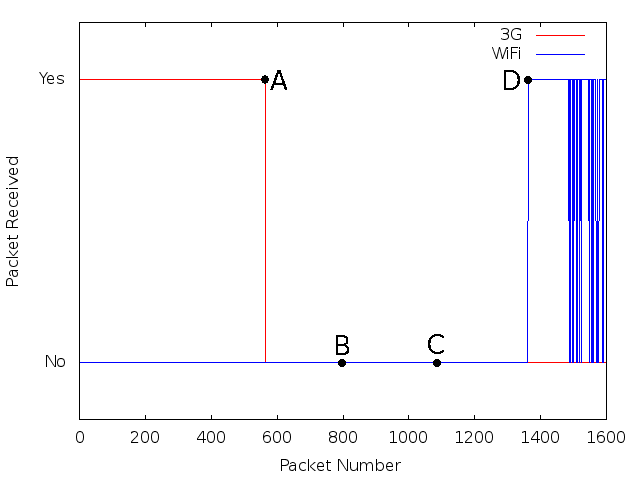
\includegraphics[width=0.5\textwidth]{paneraNoPolicy}
	\caption{TODO}
\end{figure}

Figure 2 shows, as expected, we did not receive a single packet from the time we walked within range of the WiFi to the time we attempted to access Google and accepted the store's terms and conditions. If a user left their phone in their pocket, rather than checking it as impulsively as the authors, they may never notice their phone had connected. In this case they wouldn't receive any incoming notifications until they left the store.

When run with Bouncer, the phone recieves a 302 HTTP code (a redirect to the store's terms and conditions page) after attempting to reach umich.edu. As per the implemented Bouncer policy, the phone then disconnects and reverts to the cell network. Figure 3 shows our drastically reduced downtime, present only because our implementation limits us from checking a WiFi network's Internet connection before the OS tears down the mobile connection.

\begin{figure}
	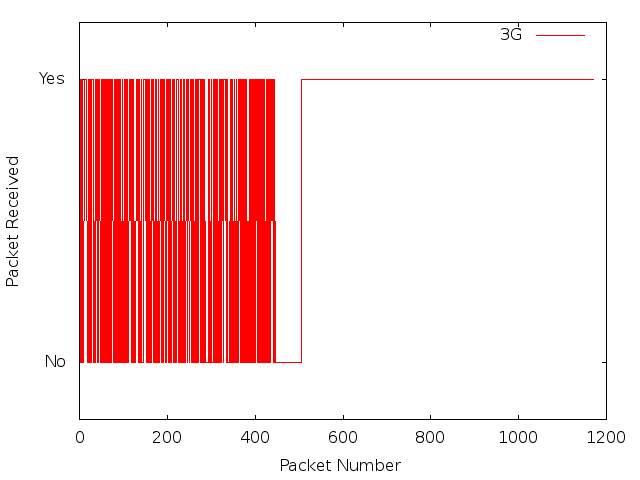
\includegraphics[width=0.5\textwidth]{paneraWithPolicy}
	\caption{TODO}
\end{figure}

\subsection{Predictive WiFi Abandonment - The Courtyards Test}
[TODO: Have Kevin check that this is a good description]
To evaluate our policy for disconnecting from poor WiFi connection, we began in a WiFi network which the authors had experienced disconnection issues from. From a starting position, connected to WiFi, we took a set route, leaving the range of the network. The route took us well out of the range of the access point, testing the transition from WiFi to cellular data.

The stock policy resulted in little to no connectivity at the perimeter of the network range. As seen in figure 4, a substantial number of packets are dropped before finally transitioning to the cellular connection. Another burst of packets are lost shortly after, when the phone tries to reconnect to the network it just left. This demonstrates a pattern the authors experienced which interrupts streaming content, and provides a generally poor user experience.

\begin{figure}
	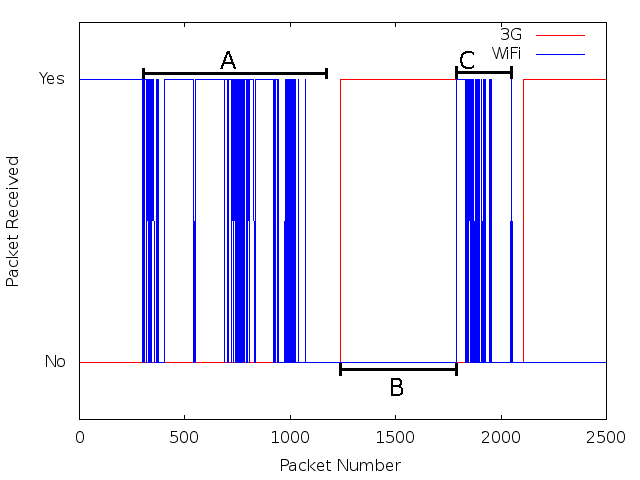
\includegraphics[width=0.5\textwidth]{leavingCourtyardsNoPolicy}
	\caption{TODO}
\end{figure}

When run with the Abandon Ship policy, as demonstrated by figure 5, the phone disconnects much more promptly from WiFi. It then stays on the cell network maintaining a stable connection. 

\begin{figure}
	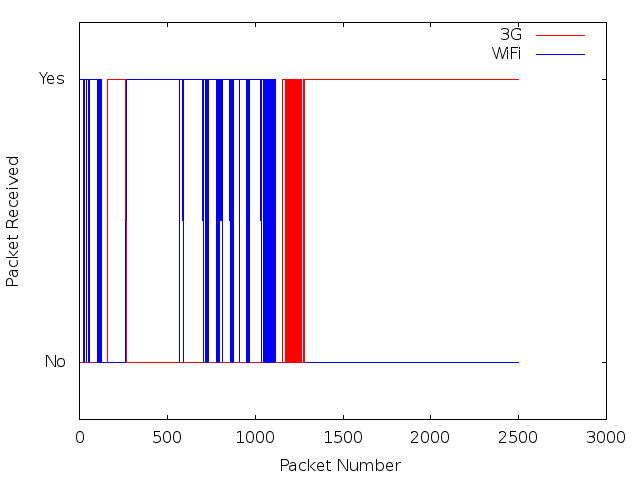
\includegraphics[width=0.5\textwidth]{leavingCourtyardsWithPolicy}
	\caption{TODO}
\end{figure}

%\begin{figure}
%	\includegraphics[width=0.5\textwidth]{}
%	\caption{TODO}
%\end{figure}